


In diesem Abschnitt sind aktuell einige Unterlagen eingefügt, die im Rahmen des Projektes eine Relevanz hatten. Vor Abgabe der Projektarbeit, soll dieser Abschnitt überarbeitet, ausgedünnt und ergänzt werden. 

\section{Projektnotizen}

Austausch und Zusammenarbeite erfolgte auf verschiedenen Platformen:
\begin{itemize}
    \item Gezeichnet und Entwürfe wurden meist in Miro erstellt: \url{https://miro.com/app/board/uXjVOdN2haQ=/}. 
    \item Besprechungen erfolgten meist in Teams: \url{https://teams.microsoft.com/l/team/19%3aDoBvOwOIC6WNhsL9kOIYFKNtVftU1yBtcEn_gcyQtcg1%40thread.tacv2/conversations?groupId=850a22ff-34a2-4fe2-a506-f55ac4d595f8&tenantId=b9b6f99a-a243-422d-ab36-f726574c981a}. 
    \item Der gemeinsame Code und die Dokumentation wurden auf Github erstelt: \url{https://github.com/tstsrv-de/tstsrv-de}. 
\end{itemize}

\subsection{Projektbesprechungen}

Stets Sonntags erfolgten Projektbesprechungen. Notizen und Zusammenfassungen davon finden sich hier in fortschreitender, chronologischer Reihenfolge. Ebenso hier entsprechend einsortiert, finden sich Konzeptzeichnungen und Entwürfe aller Art (UI, Code, Datenbankmodelle).

(TODO!) Bildbeschreibungen ergänzen, wichtige Bilder beschreiben.

2021-11-23-erster-entwurf-gameloop 
\begin{figure}[H]
    \centering
    \caption[]{2021-11-23-erster-entwurf-gameloop}
    \label{fig:2021-11-23-erster-entwurf-gameloop}
    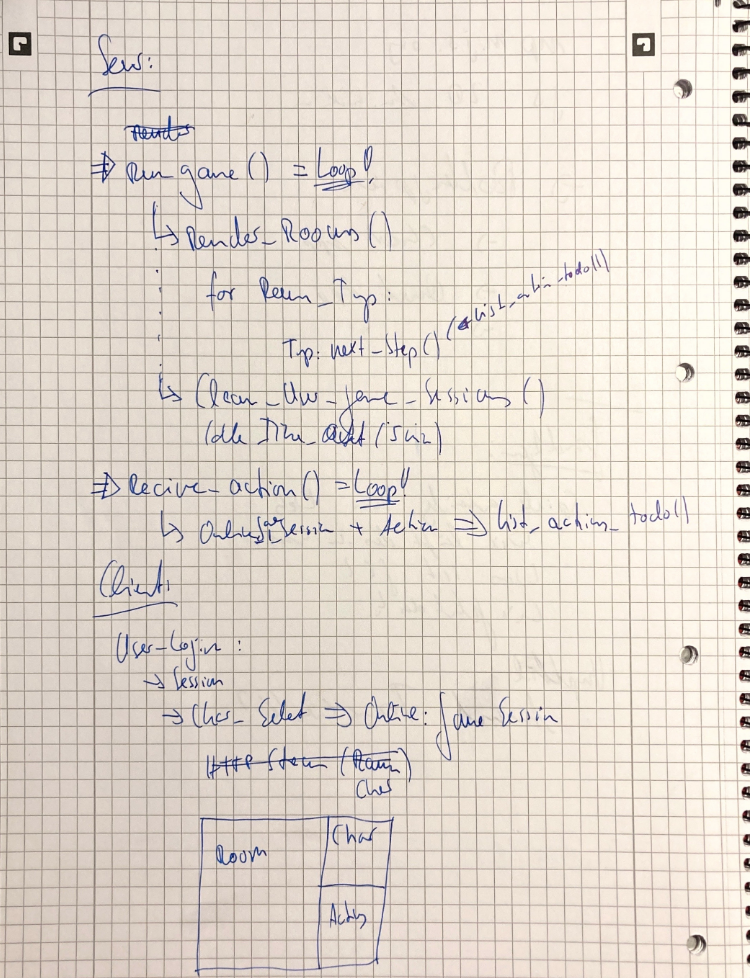
\includegraphics[width=1\textwidth]{2021-11-23-erster-entwurf-gameloop}
\end{figure}

2021-11-23-erstes-db-konzept 
\begin{figure}[H]
    \centering
    \caption[]{2021-11-23-erstes-db-konzept}
    \label{fig:2021-11-23-erstes-db-konzept}
    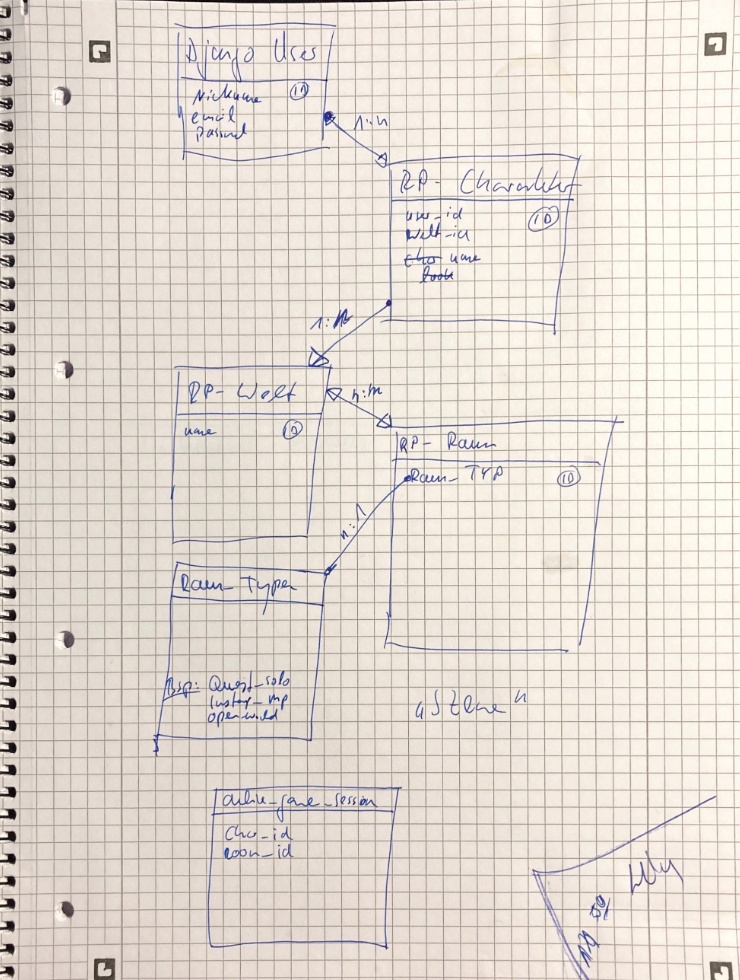
\includegraphics[width=1\textwidth]{2021-11-23-erstes-db-konzept}
\end{figure}

2021-11-27-erstentwurf-ui 
\begin{figure}[H]
    \centering
    \caption[]{2021-11-27-erstentwurf-ui}
    \label{fig:2021-11-27-erstentwurf-ui}
    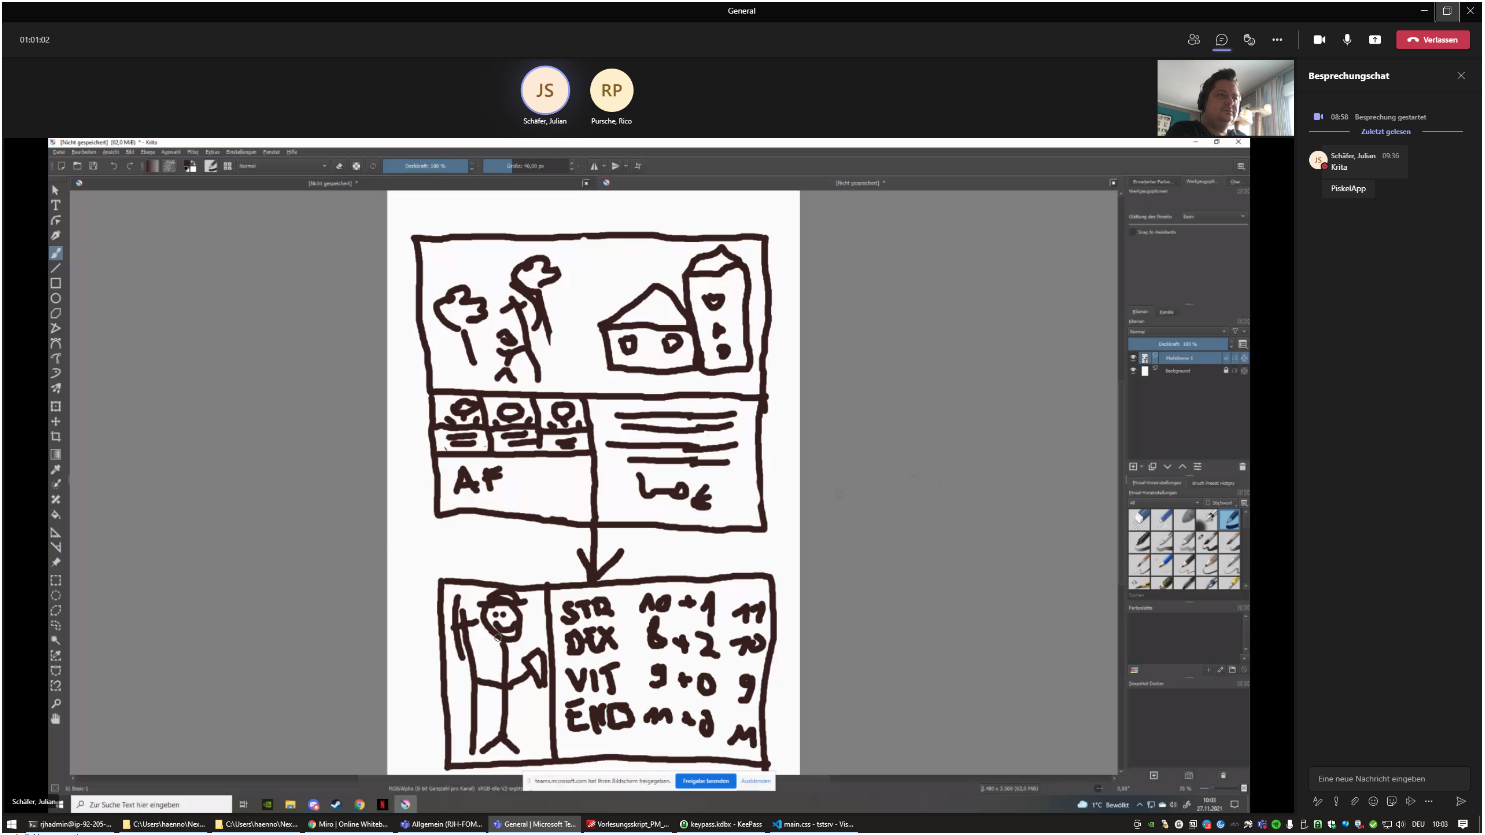
\includegraphics[width=1\textwidth]{2021-11-27-erstentwurf-ui}
\end{figure}

2021-11-27-projektskizze-1 
\begin{figure}[H]
    \centering
    \caption[]{2021-11-27-projektskizze-1}
    \label{fig:2021-11-27-projektskizze-1}
    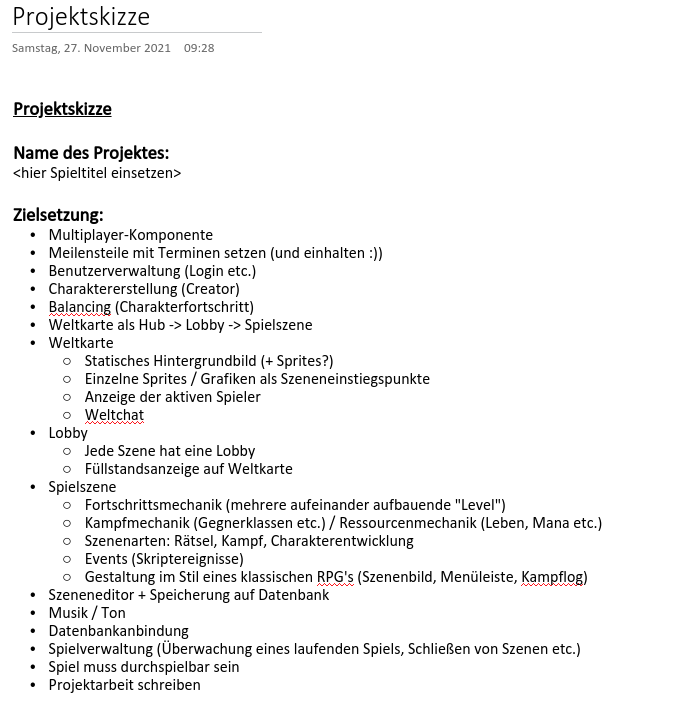
\includegraphics[width=1\textwidth]{2021-11-27-projektskizze-1}
\end{figure}

2021-11-27-projektskizze-2 
\begin{figure}[H]
    \centering
    \caption[]{2021-11-27-projektskizze-2}
    \label{fig:2021-11-27-projektskizze-2}
    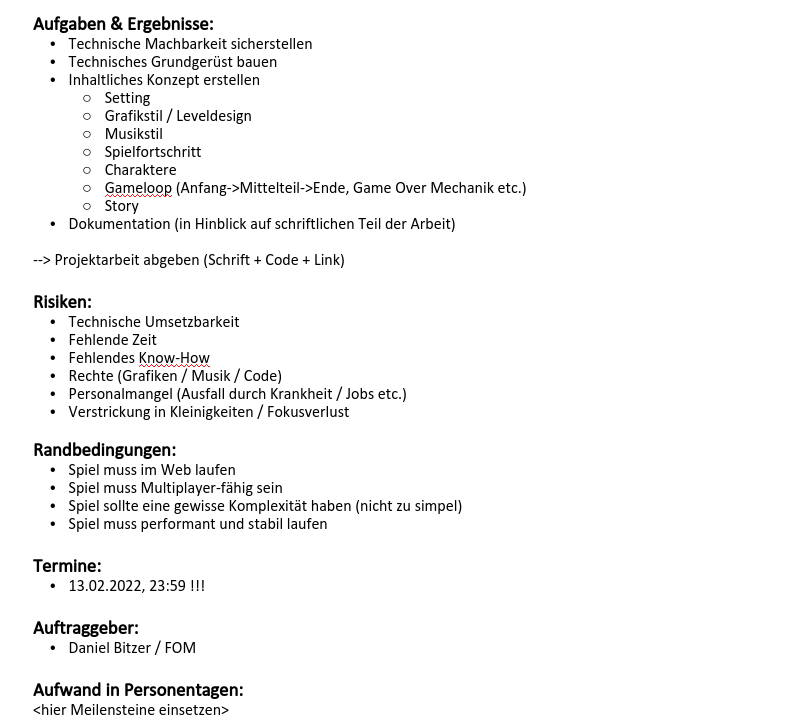
\includegraphics[width=1\textwidth]{2021-11-27-projektskizze-2}
\end{figure}

2021-11-29-Entwurf-Klassen-Ui 
\begin{figure}[H]
    \centering
    \caption[]{2021-11-29-Entwurf-Klassen-Ui}
    \label{fig:2021-11-29-Entwurf-Klassen-Ui}
    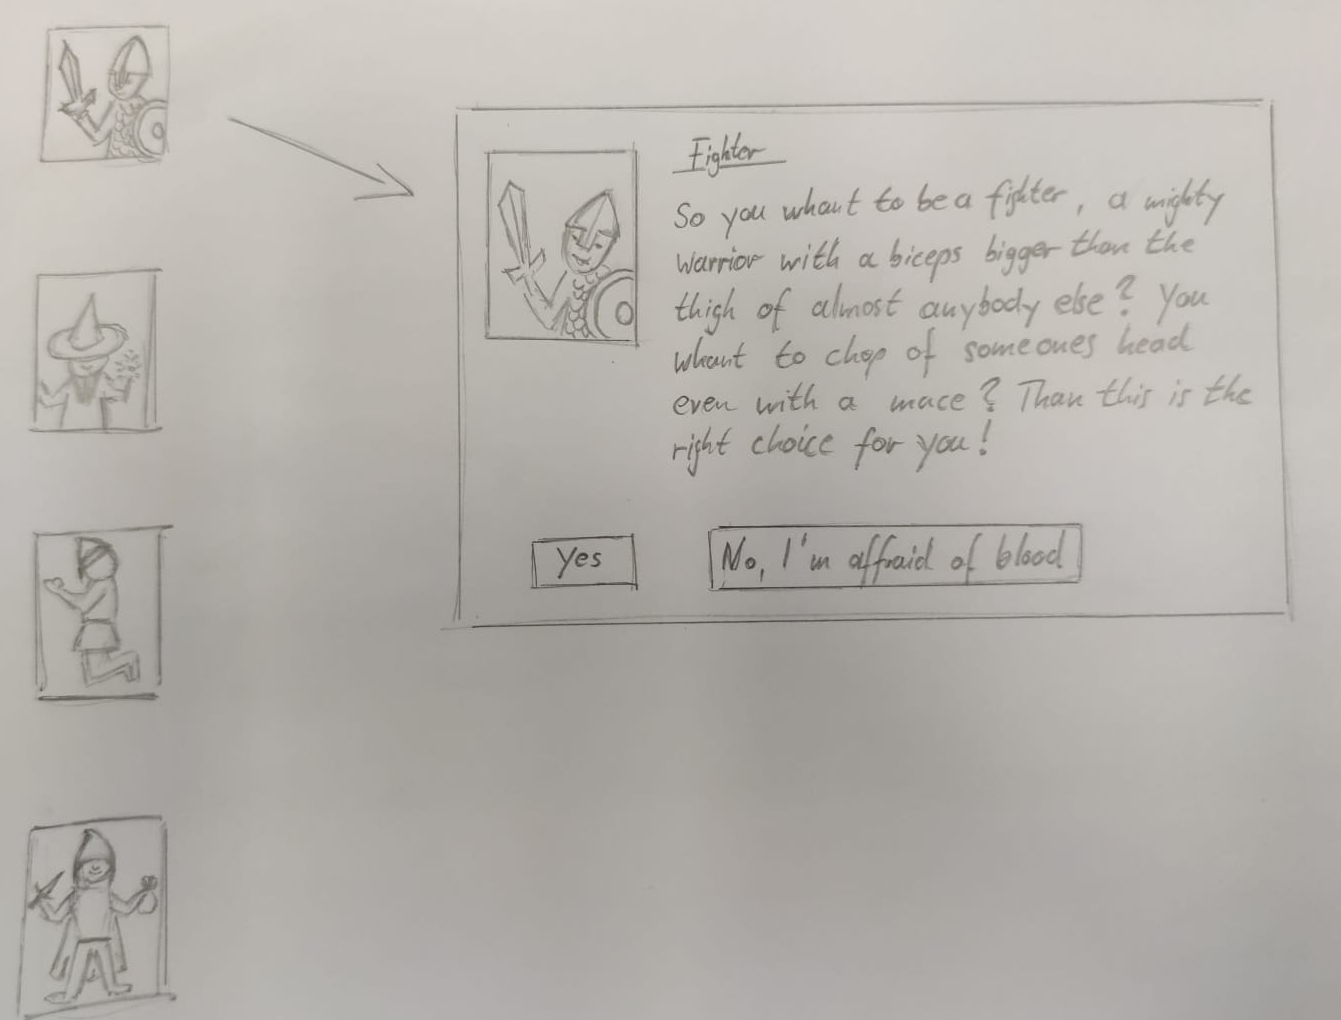
\includegraphics[width=1\textwidth]{2021-11-29-Entwurf-Klassen-Ui}
\end{figure}

2021-11-30-Entwurf-Lobby-Logik 
\begin{figure}[H]
    \centering
    \caption[]{2021-11-30-Entwurf-Lobby-Logik}
    \label{fig:2021-11-30-Entwurf-Lobby-Logik}
    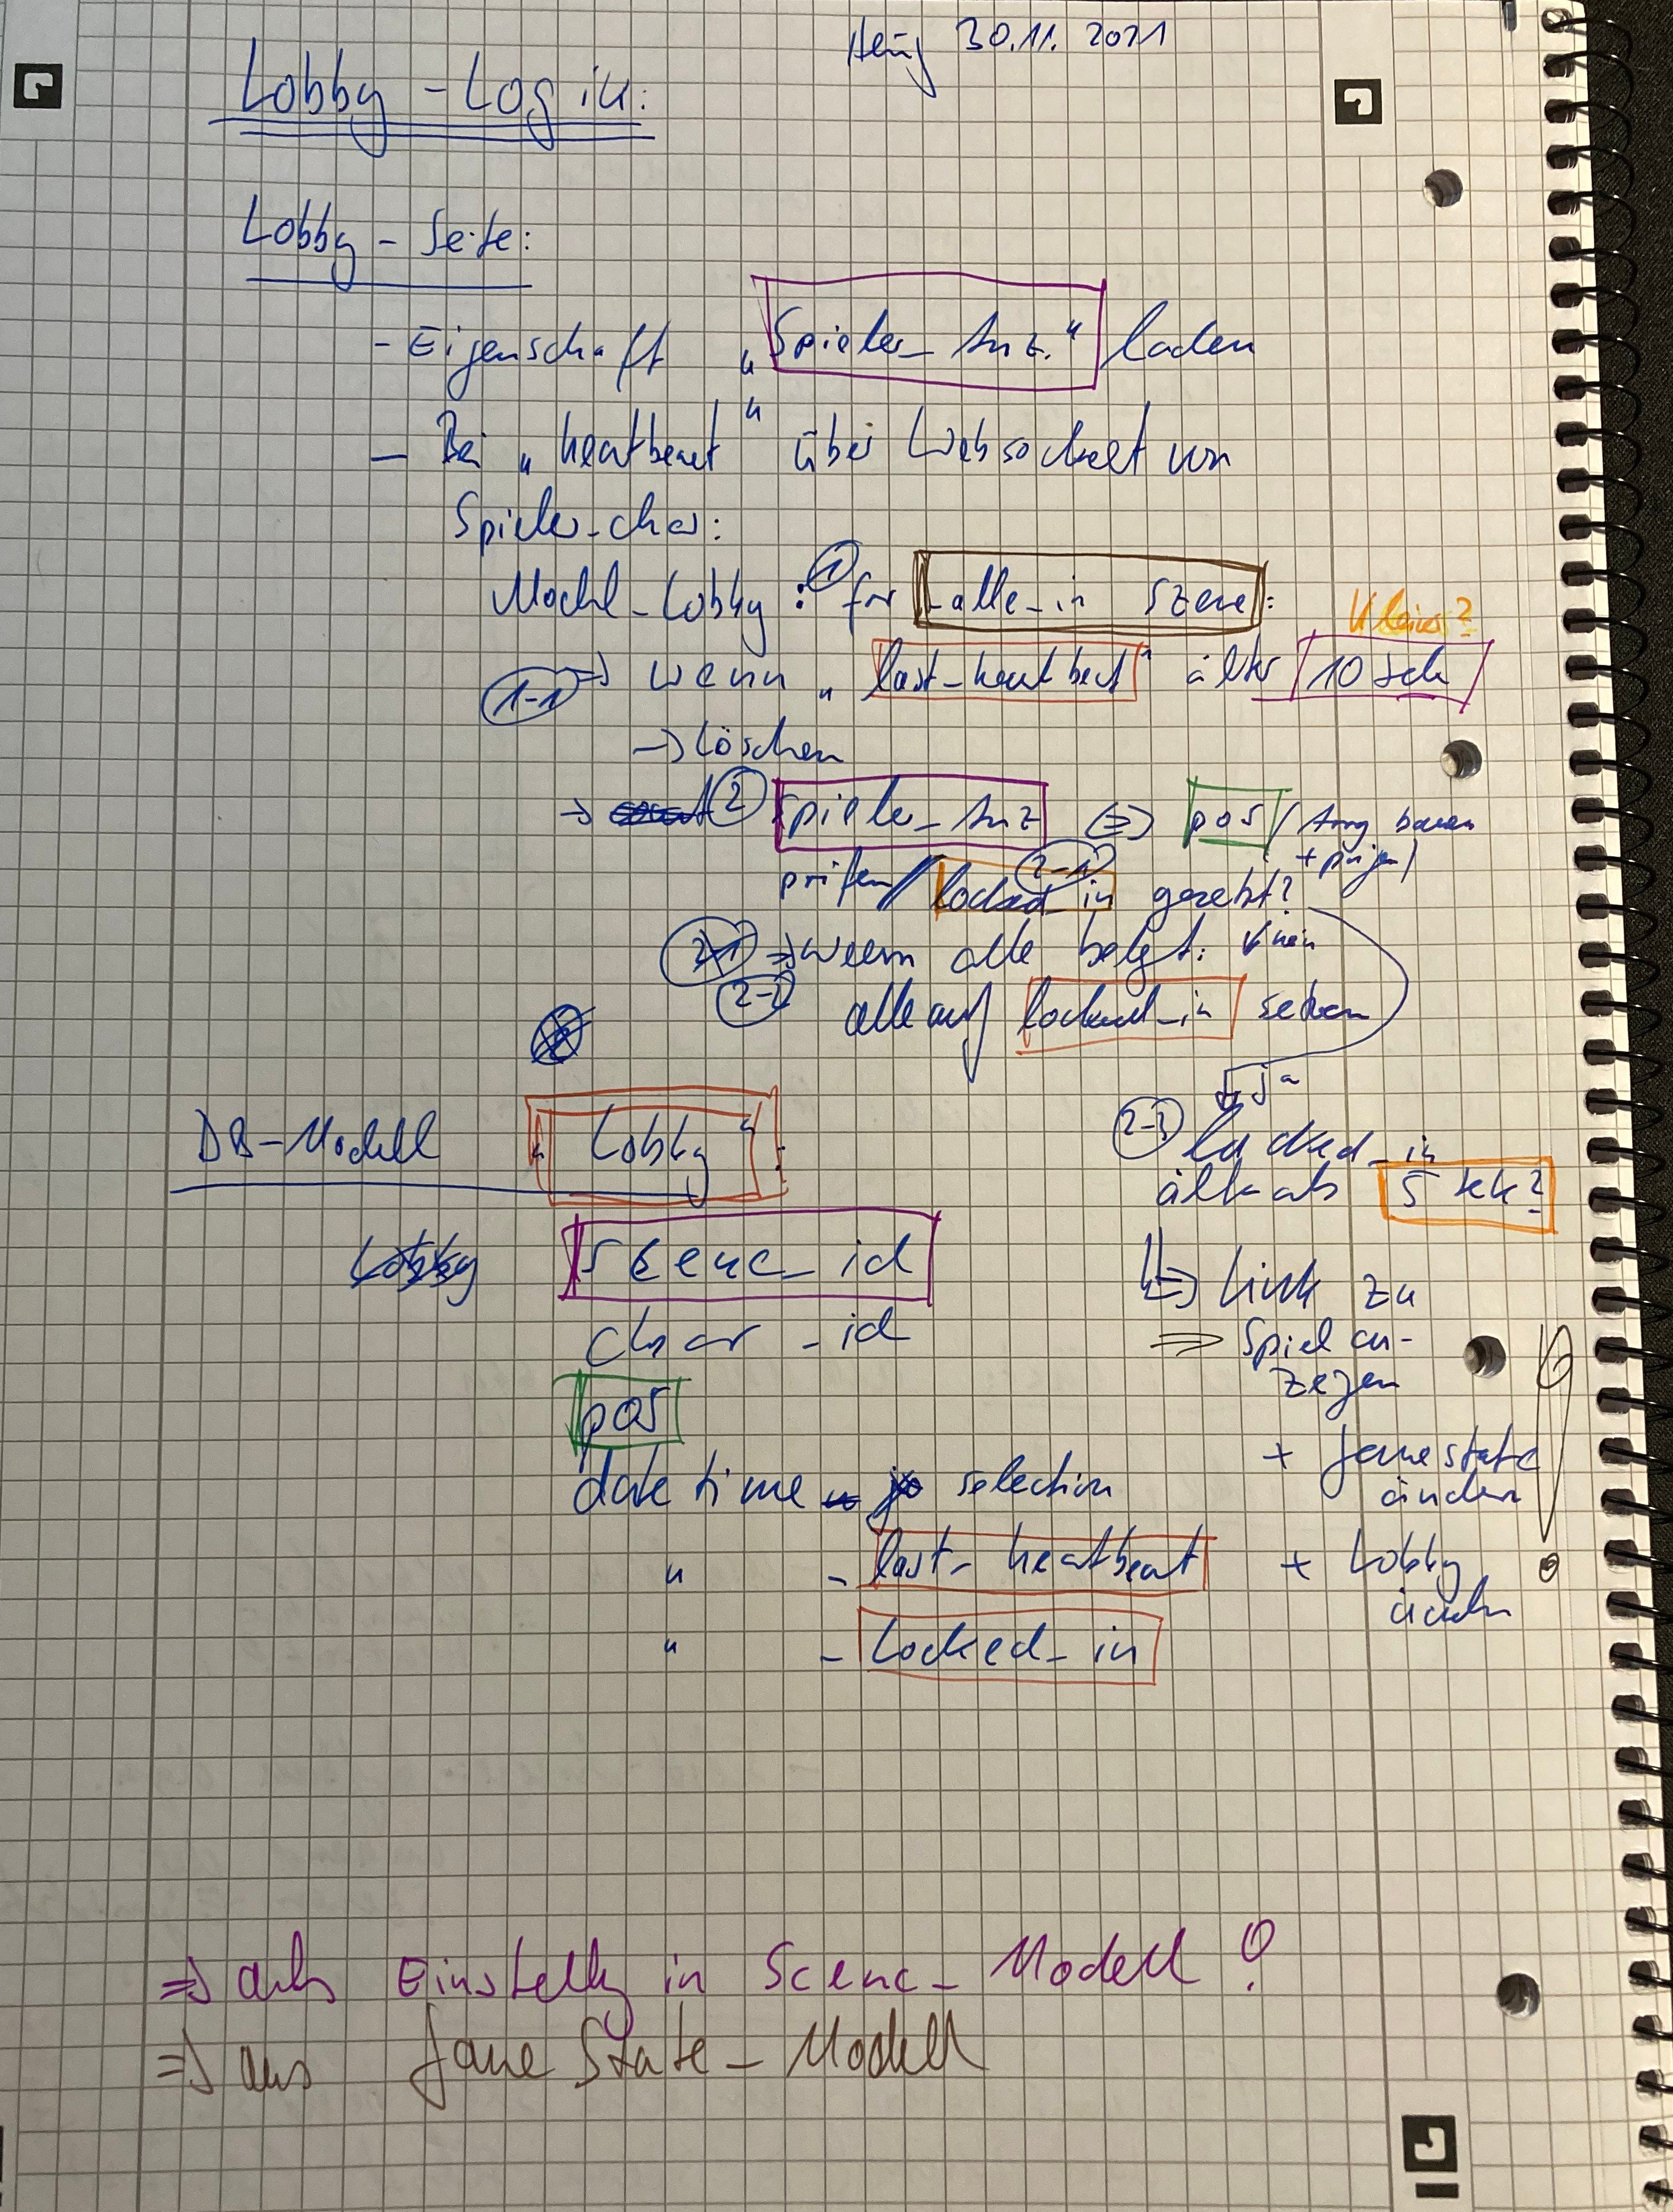
\includegraphics[width=1\textwidth]{2021-11-30-Entwurf-Lobby-Logik}
\end{figure}

2021-11-30-Entwurf-Lobby-UI 
\begin{figure}[H]
    \centering
    \caption[]{2021-11-30-Entwurf-Lobby-UI}
    \label{fig:2021-11-30-Entwurf-Lobby-UI}
    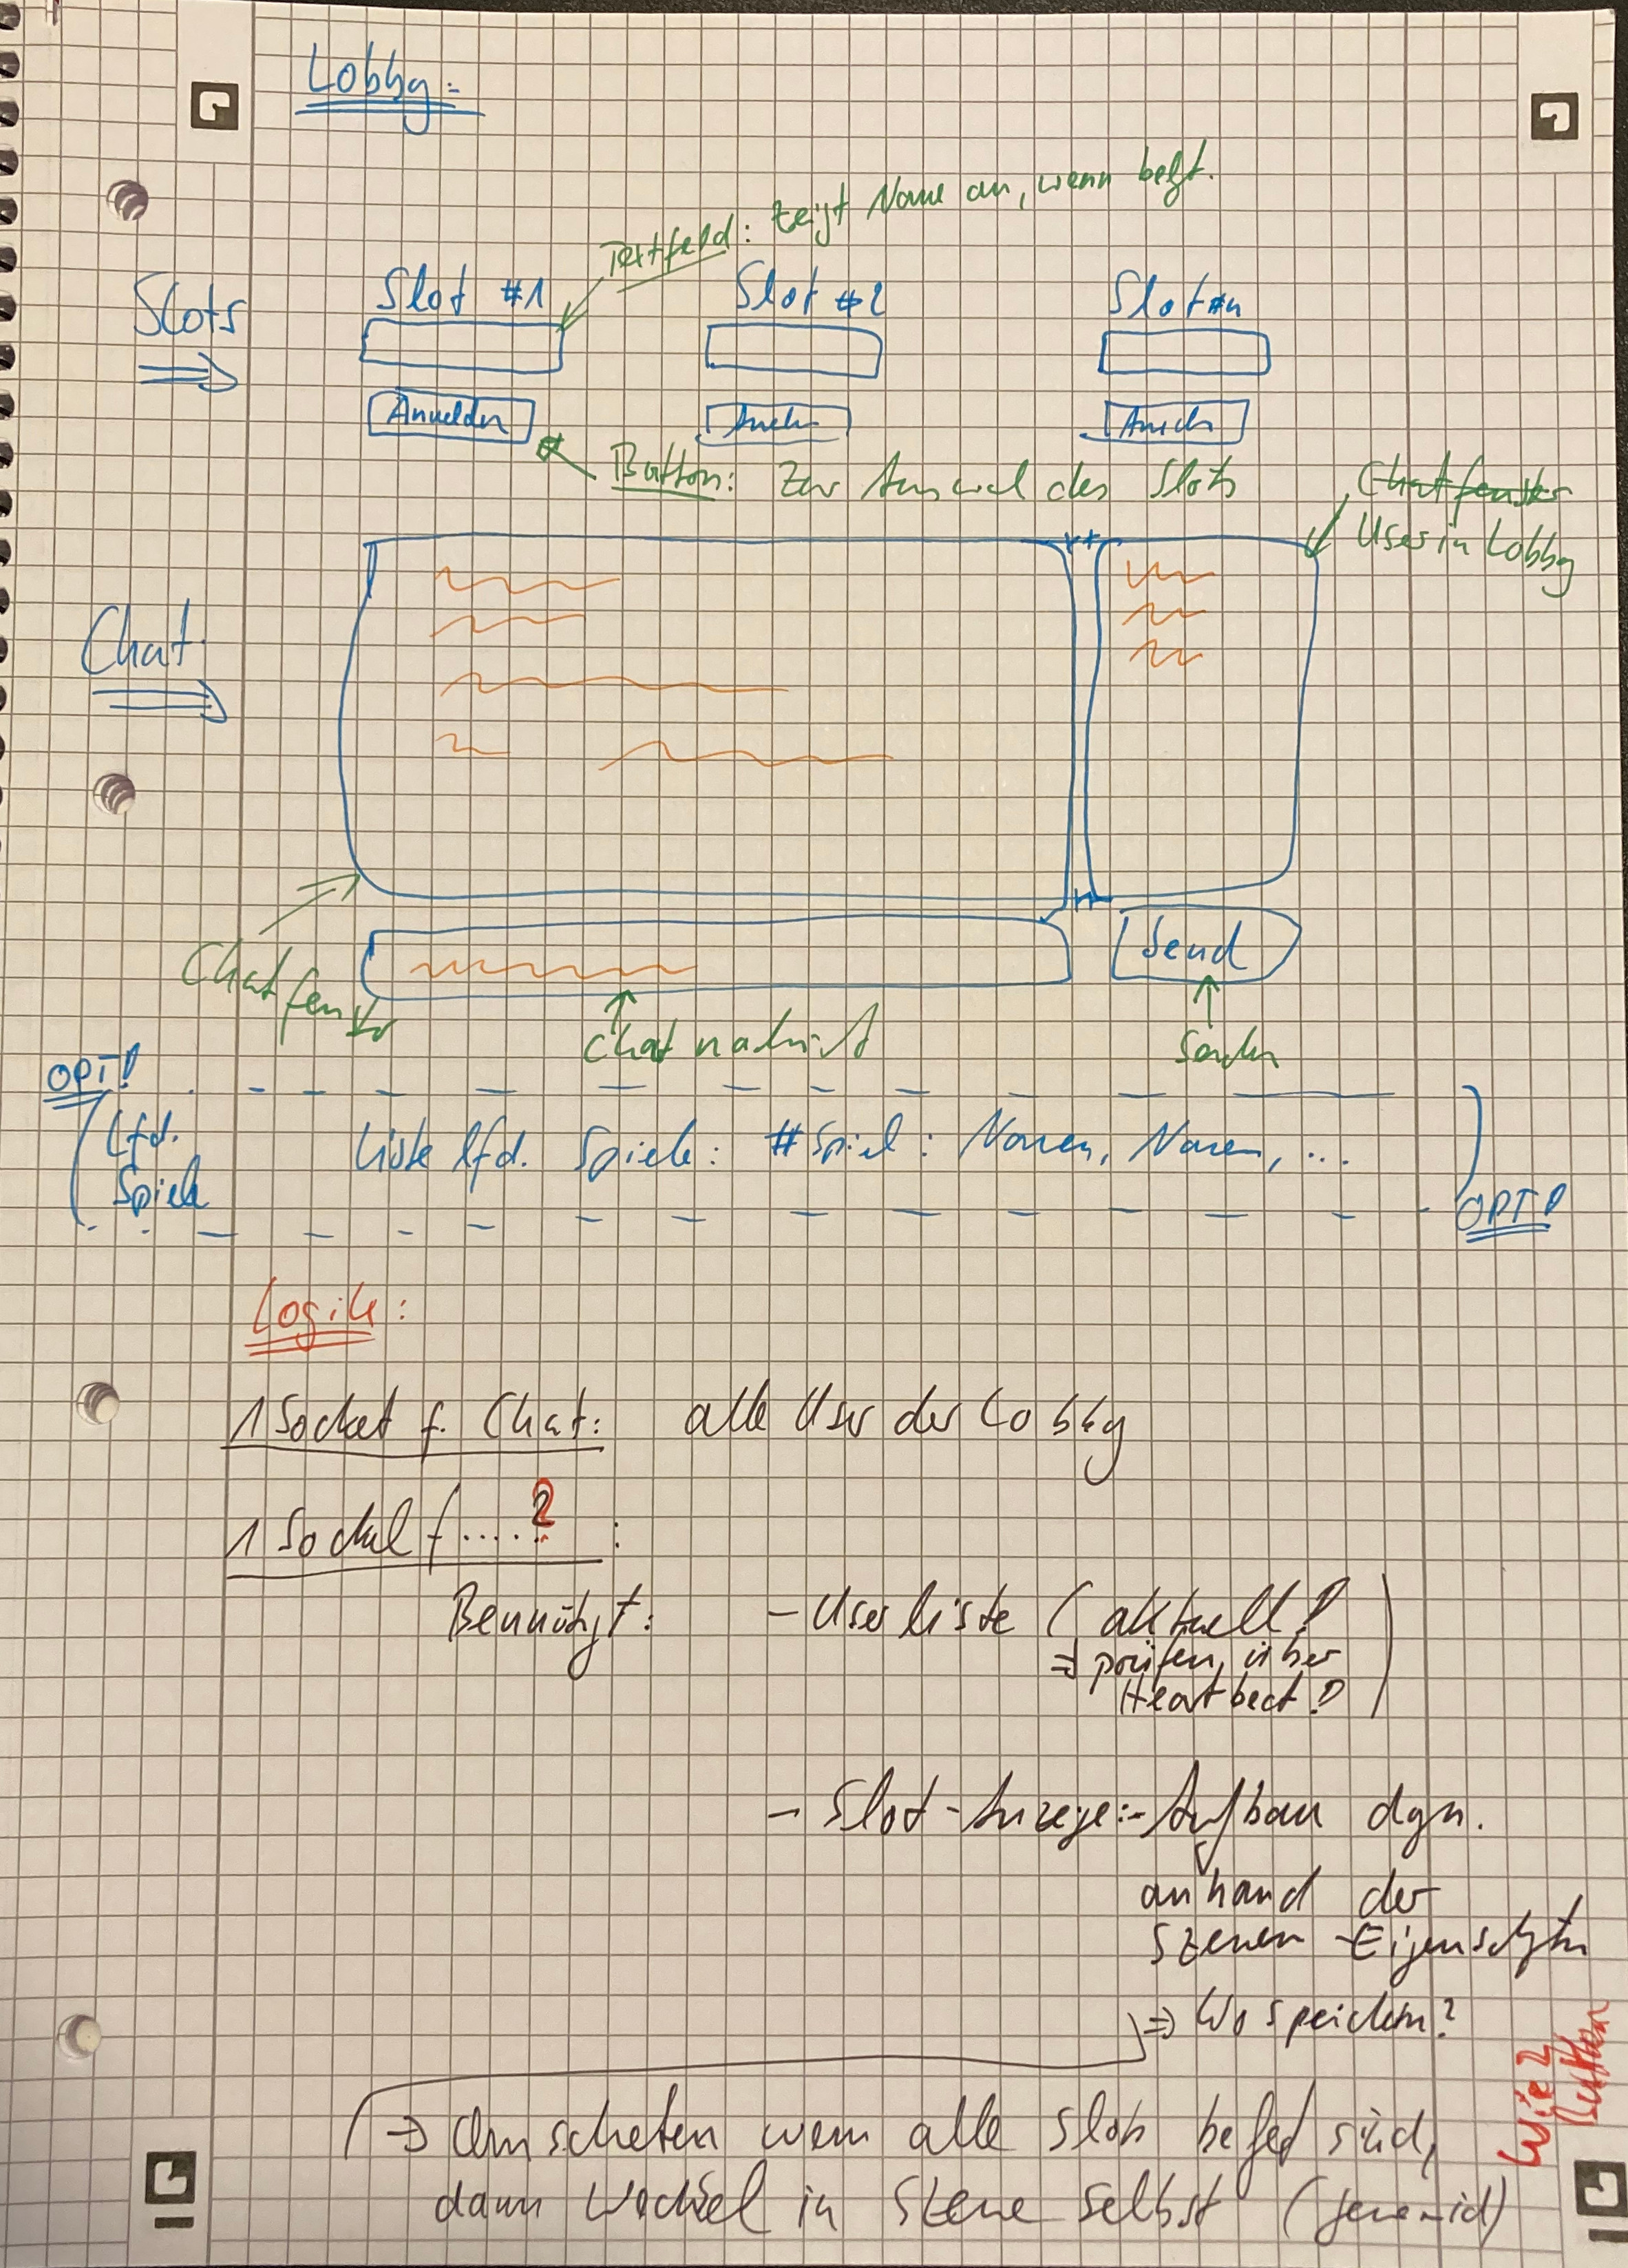
\includegraphics[width=1\textwidth]{2021-11-30-Entwurf-Lobby-UI}
\end{figure}

2021-12-02-Countdown-Logik 
\begin{figure}[H]
    \centering
    \caption[]{2021-12-02-Countdown-Logik}
    \label{fig:2021-12-02-Countdown-Logik}
    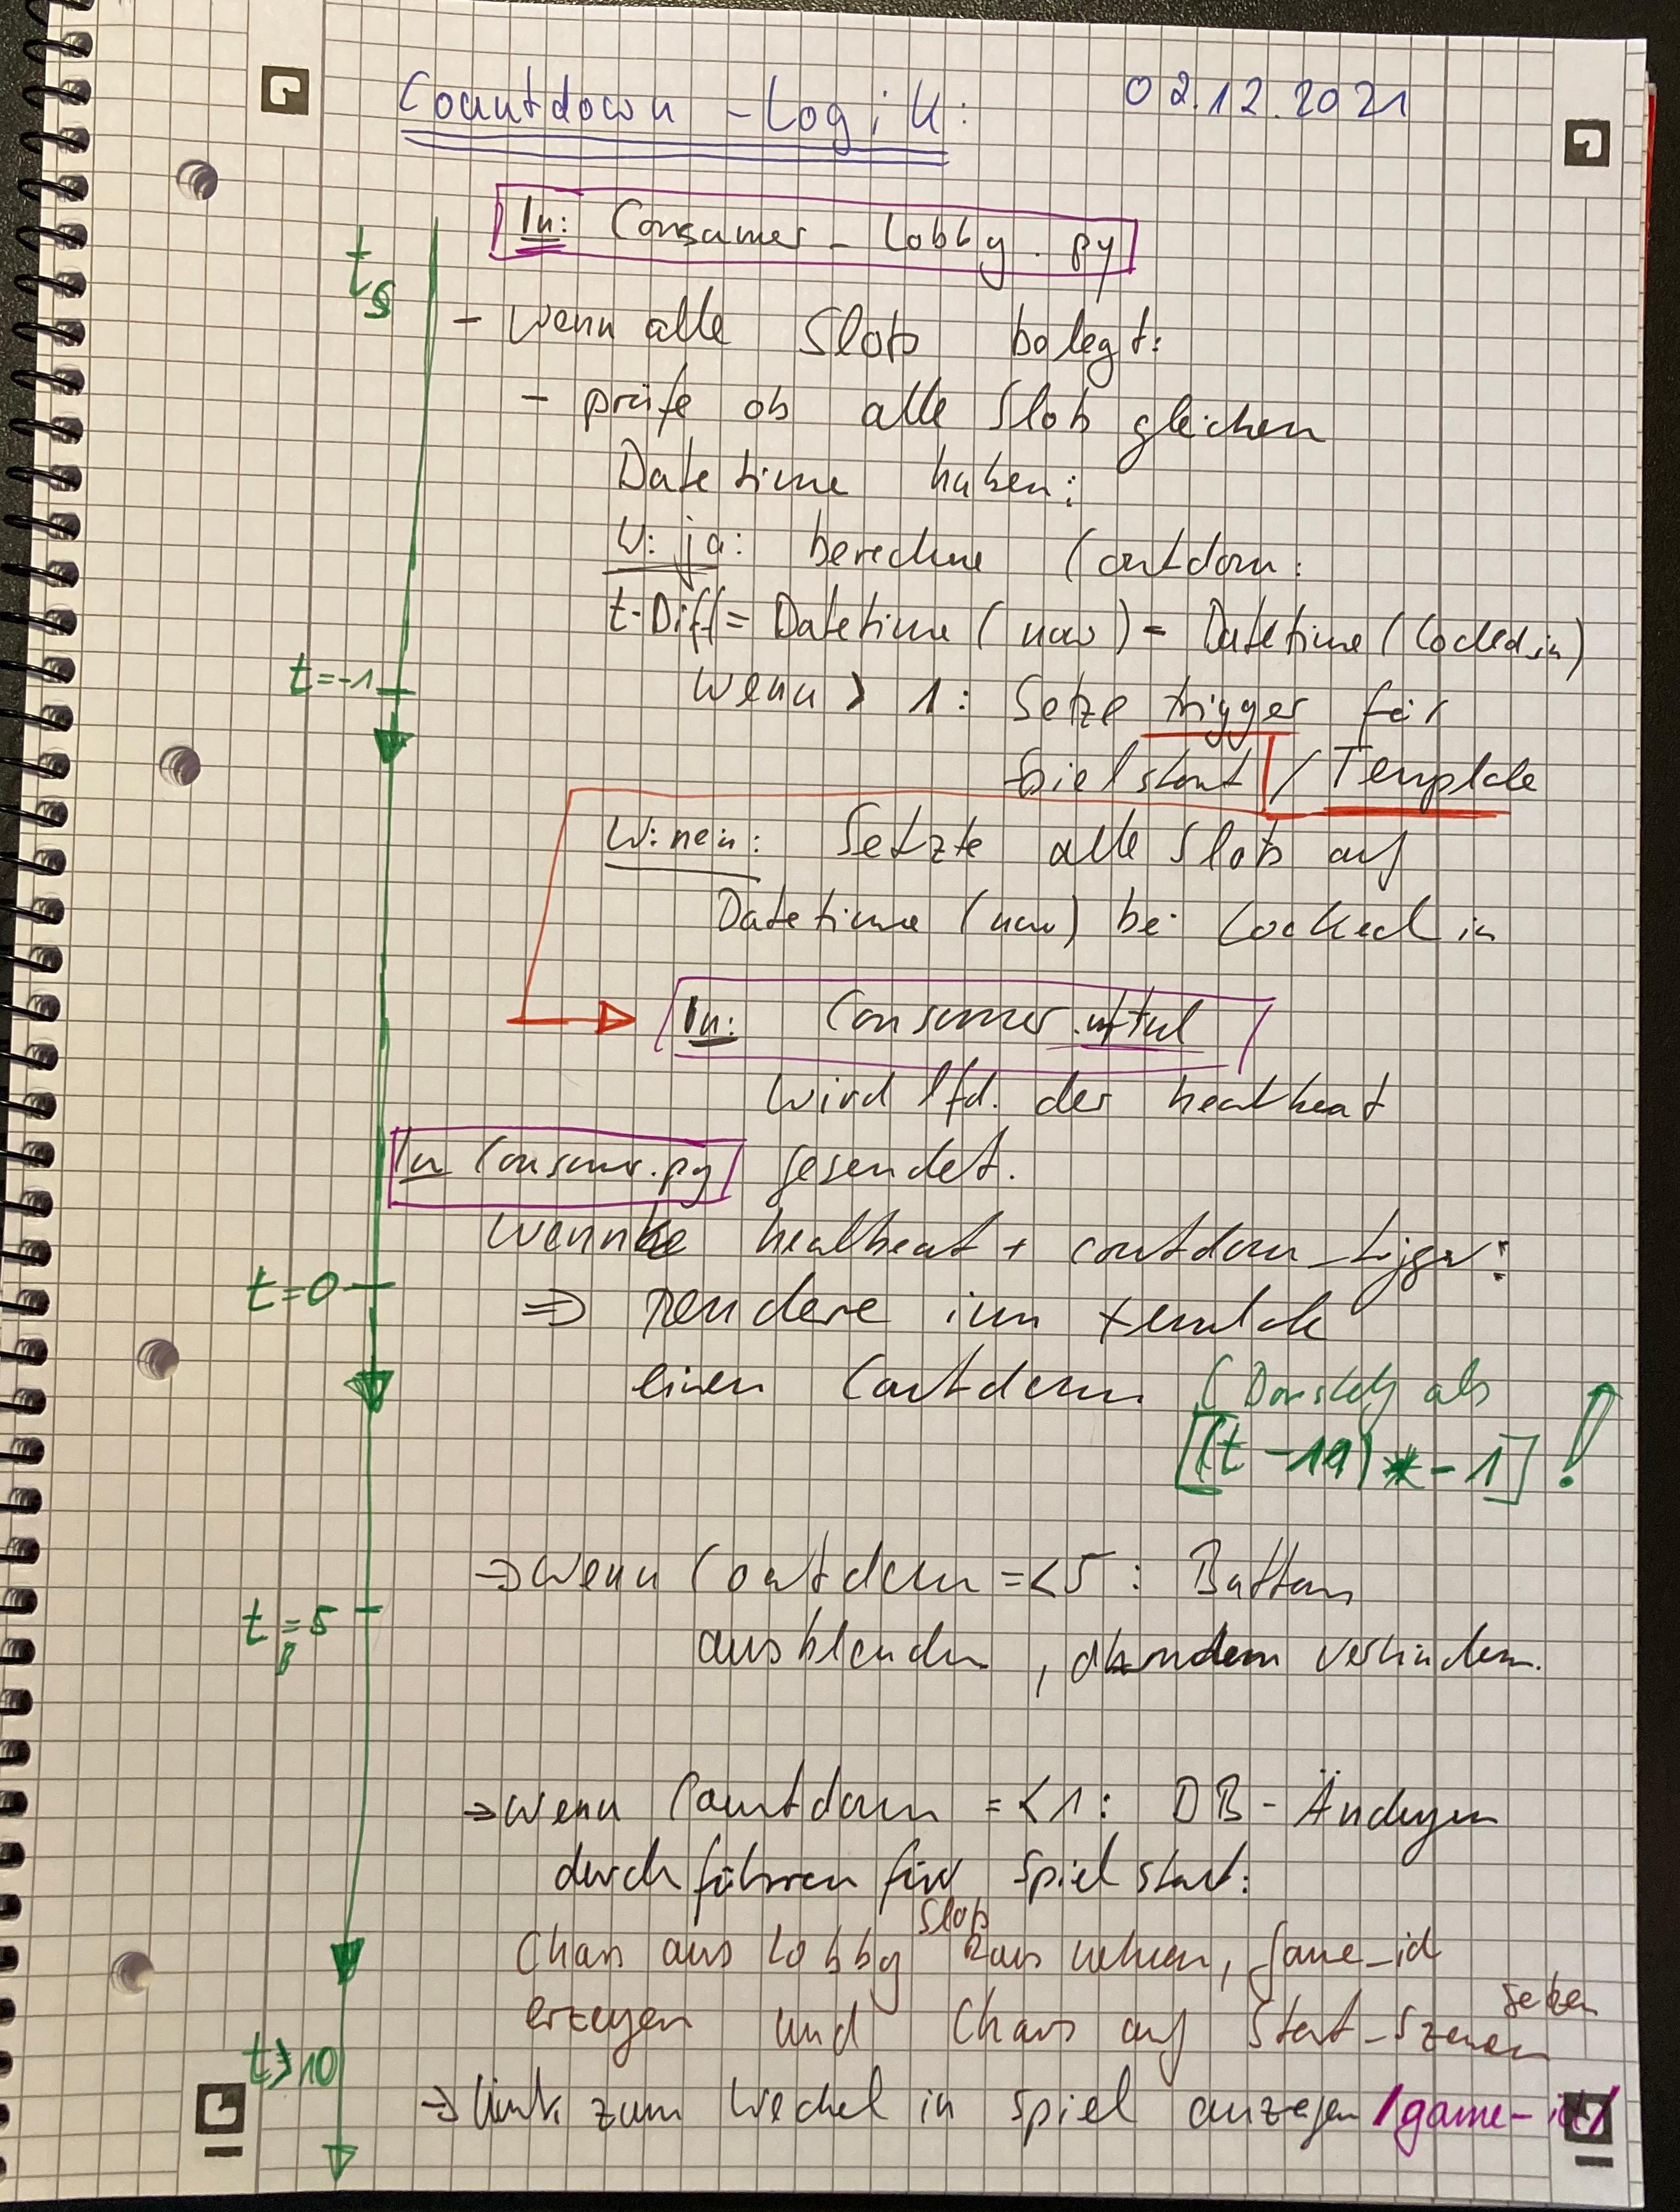
\includegraphics[width=1\textwidth]{2021-12-02-Countdown-Logik}
\end{figure}

2021-12-05-Projketbesprechung-Miro-b 
\begin{figure}[H]
    \centering
    \caption[]{2021-12-05-Projketbesprechung-Miro-b}
    \label{fig:2021-12-05-Projketbesprechung-Miro-b}
    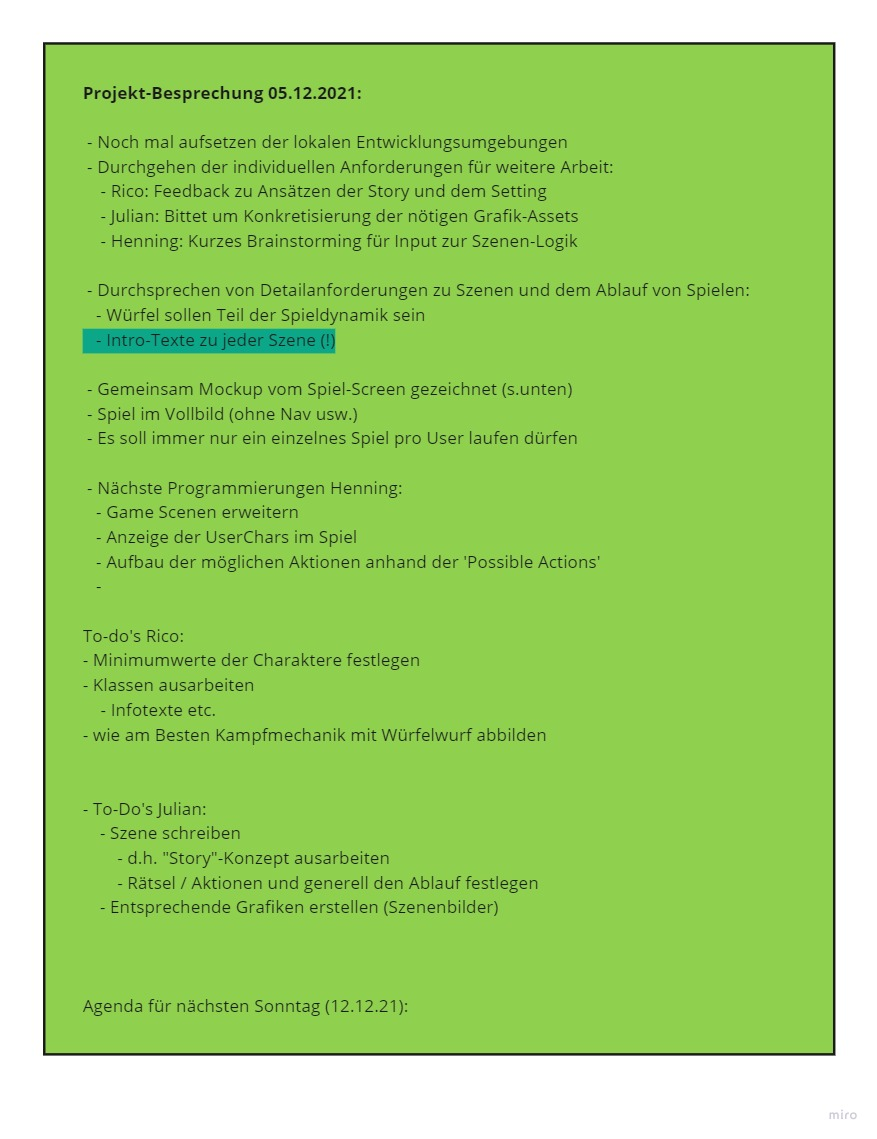
\includegraphics[width=1\textwidth]{2021-12-05-Projketbesprechung-Miro-b}
\end{figure}

2021-12-05-Projketbesprechung-Miro-c 
\begin{figure}[H]
    \centering
    \caption[]{2021-12-05-Projketbesprechung-Miro-c}
    \label{fig:2021-12-05-Projketbesprechung-Miro-c}
    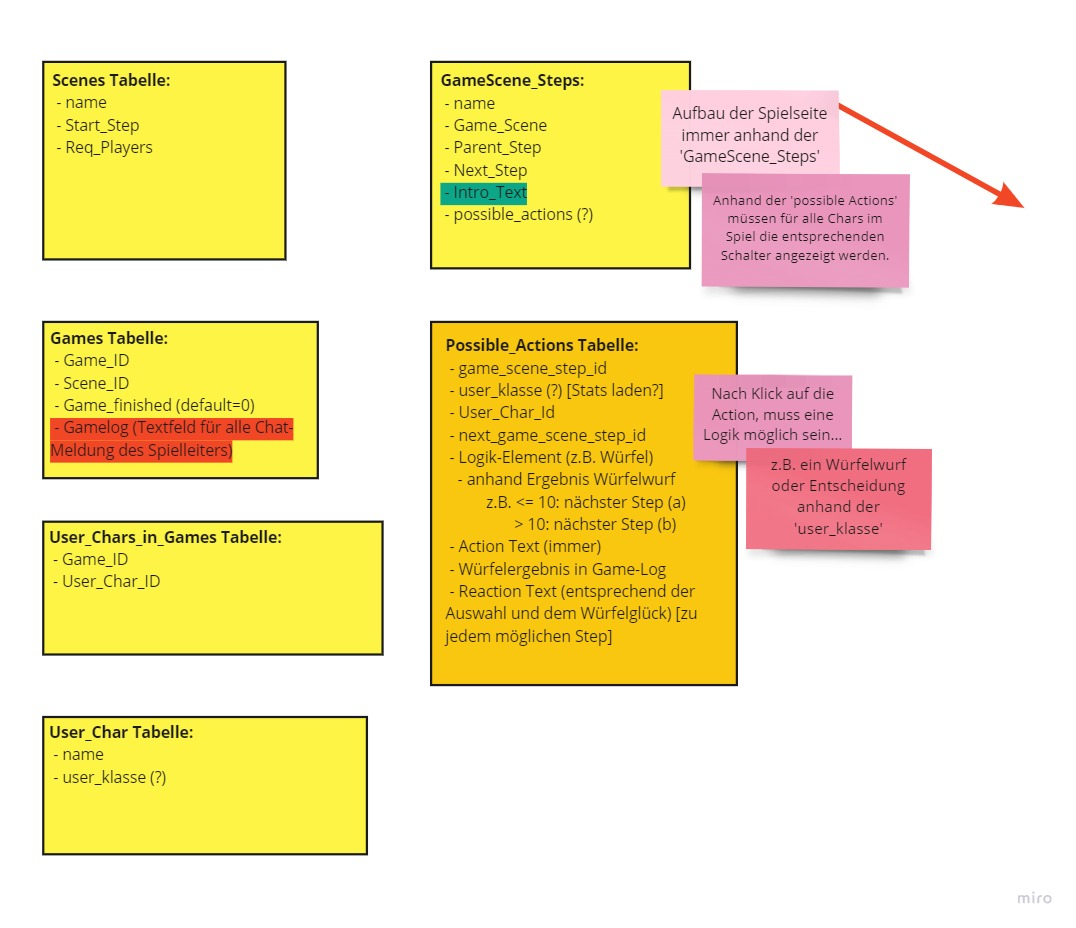
\includegraphics[width=1\textwidth]{2021-12-05-Projketbesprechung-Miro-c}
\end{figure}

2021-12-05-Projketbesprechung-Miro-d 
\begin{figure}[H]
    \centering
    \caption[]{2021-12-05-Projketbesprechung-Miro-d}
    \label{fig:2021-12-05-Projketbesprechung-Miro-d}
    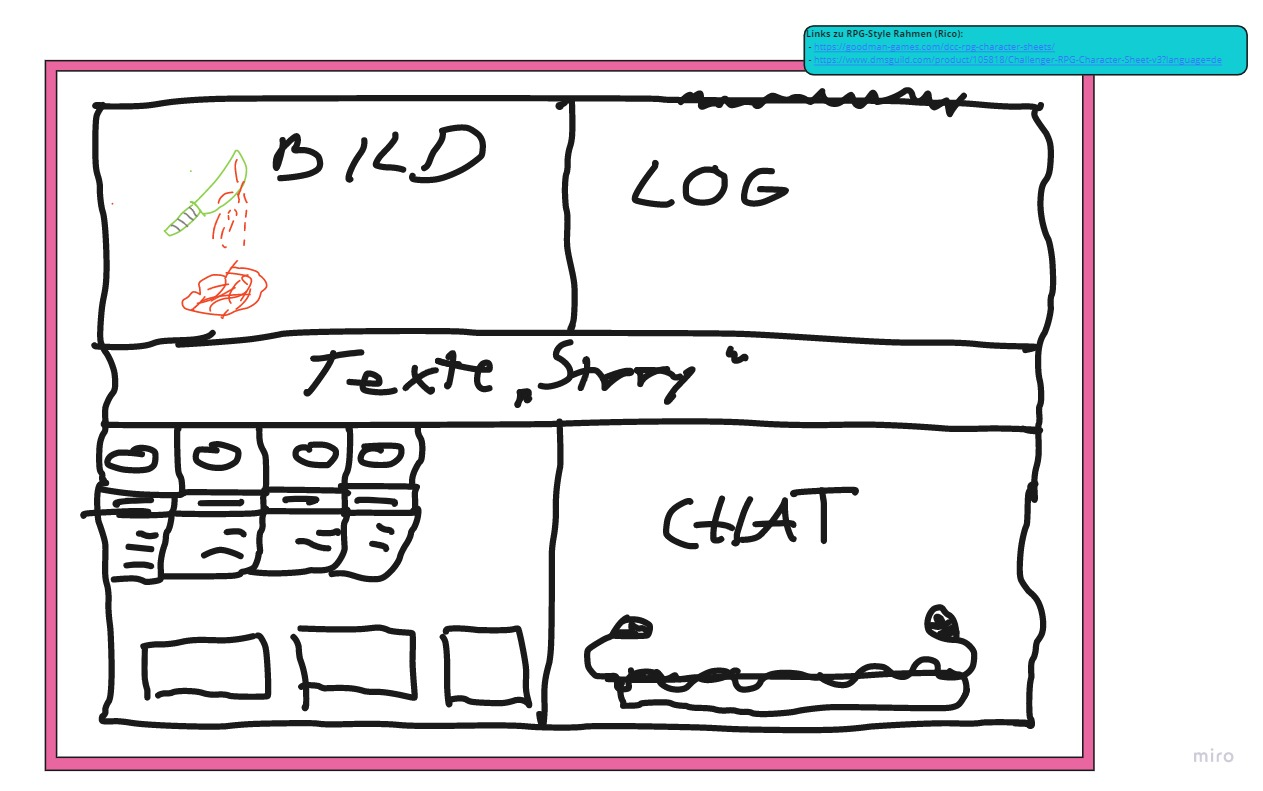
\includegraphics[width=1\textwidth]{2021-12-05-Projketbesprechung-Miro-d}
\end{figure}

2021-12-11-Projekt-Besprechung-Klassenbeschreibung 
\begin{figure}[H]
    \centering
    \caption[]{2021-12-11-Projekt-Besprechung-Klassenbeschreibung}
    \label{fig:2021-12-11-Projekt-Besprechung-Klassenbeschreibung}
    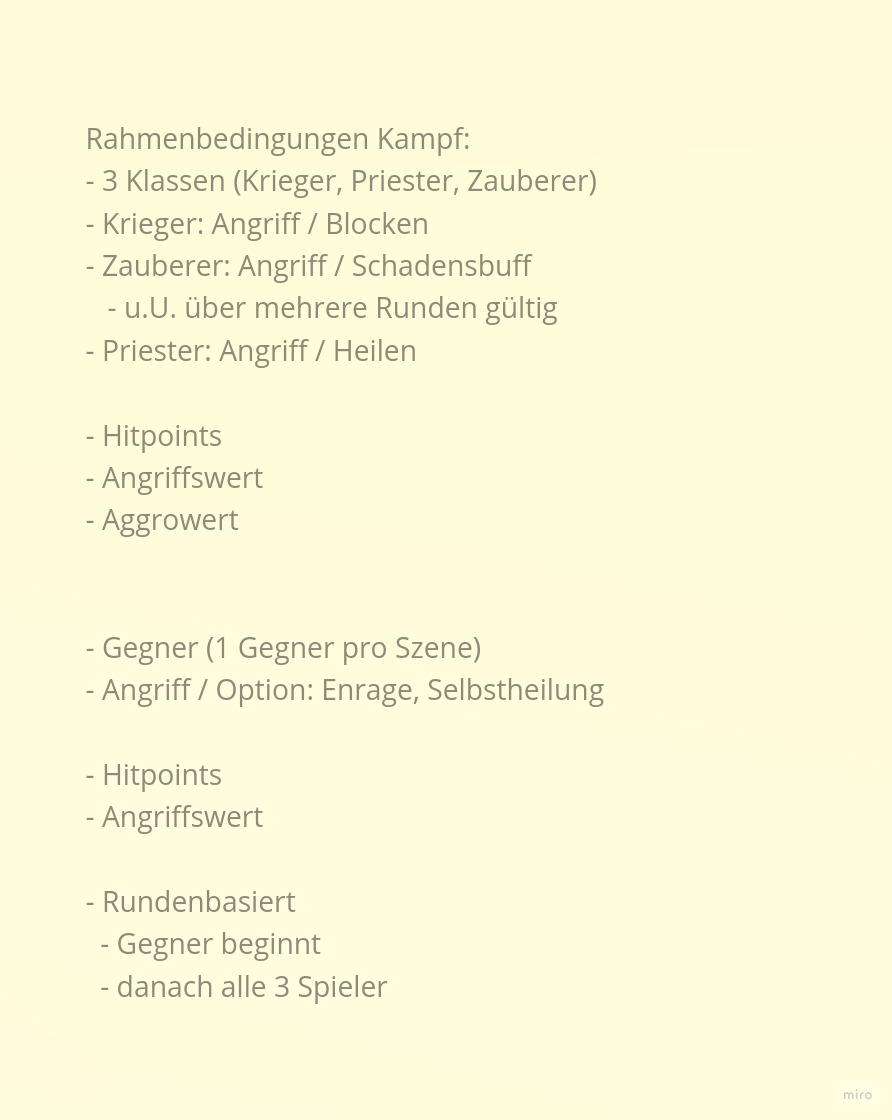
\includegraphics[width=1\textwidth]{2021-12-11-Projekt-Besprechung-Klassenbeschreibung}
\end{figure}

2021-12-11-Projekt-Besprechung 
\begin{figure}[H]
    \centering
    \caption[]{2021-12-11-Projekt-Besprechung}
    \label{fig:2021-12-11-Projekt-Besprechung}
    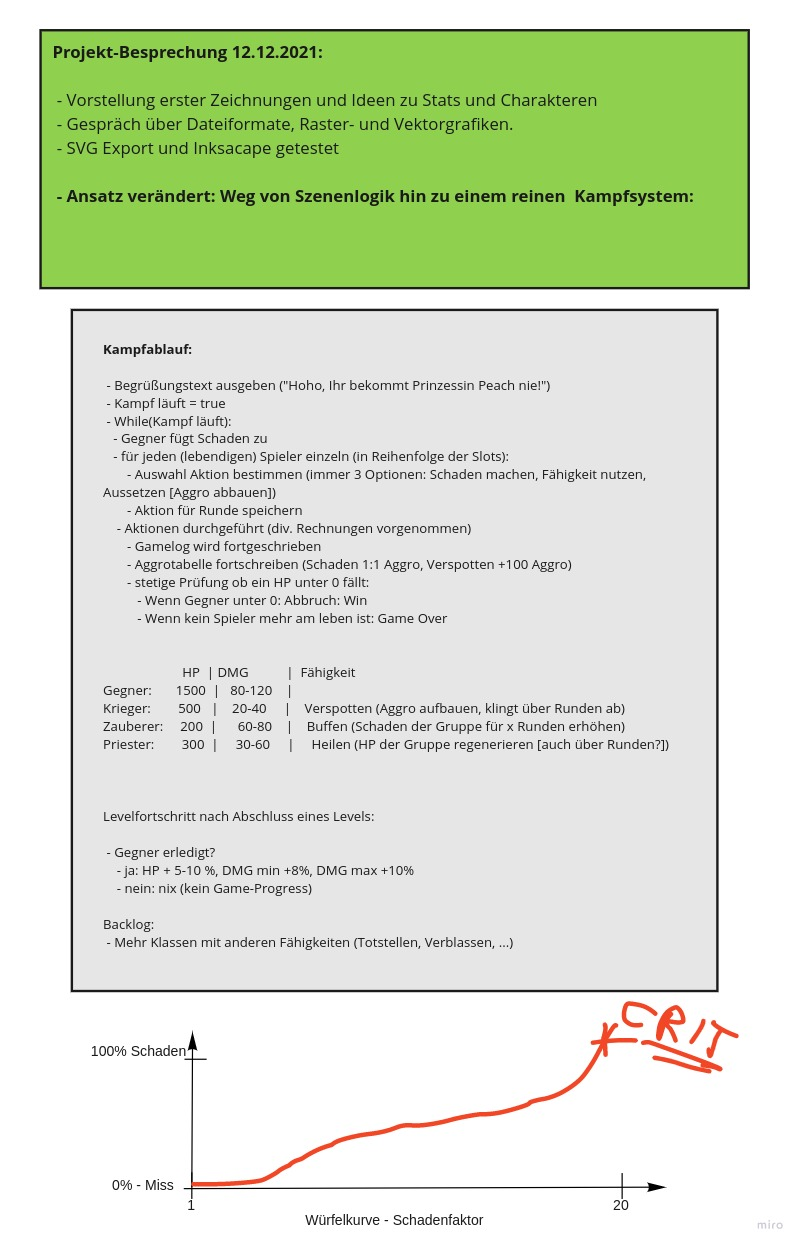
\includegraphics[width=1\textwidth]{2021-12-11-Projekt-Besprechung}
\end{figure}



\section{Entwicklungsnotizen}

\subsection{Entwicklung, Sonntag 19.12.2021:}

An diesem Tag wurden weitere, notwenige Grundlagen für die Integration der Spiellogik eingebaut. Das insbesondere in Vorbereitung auf die kommenden Anpassungen und Entwicklungen die in der Projektbesprechung vom 11.12.2021 besprochen wurden. 
Konkret: 

\begin{itemize}
	\item Prüfung auf den Seiten Chars, Worldmap und Lobby ob dieser Benutzer ein aktives Spiel hat. Falls ja, wird der Benutzer auf diese Seite umgeleitet.
	\item Grundfunktion für das Beenden von einem Spiel eingebaut: Man kann nun per Klick im Spiel, das Spiel beenden.
	\item Daran anschließend eine Prüfung im laufendem Spiel, ob das Spiele beendet wurde und falls ja, Anzeige eines Endbildschirms.
\end{itemize}

Die Entwicklung der Grundlagen an diesem Tag wurde mit Fokus auf Modularisierung erledigt. Der Code der  jeweiligen Funktionen wurde in einzelnen Dateien ausgelagert um Wiederverwendbarkeit und Lesbarkeit zu erhöhen. 

Die zugehörigen Commits sind insbesondere: 
\url{https://github.com/tstsrv-de/tstsrv-de/commit/b43f7f42182007ced4fcb8f07e64545769650c0a} und 
\url{https://github.com/tstsrv-de/tstsrv-de/commit/175ef5601ac029669252832a6645cf35ac422afa}




\begin{figure}[H]
    \centering
    \caption[]{Projektbesprechung vom 11.12.2021, Details zu den Klassen}
	\label{fig:Projektbesprechung vom 11.12.2021, Details zu den Klassen}
    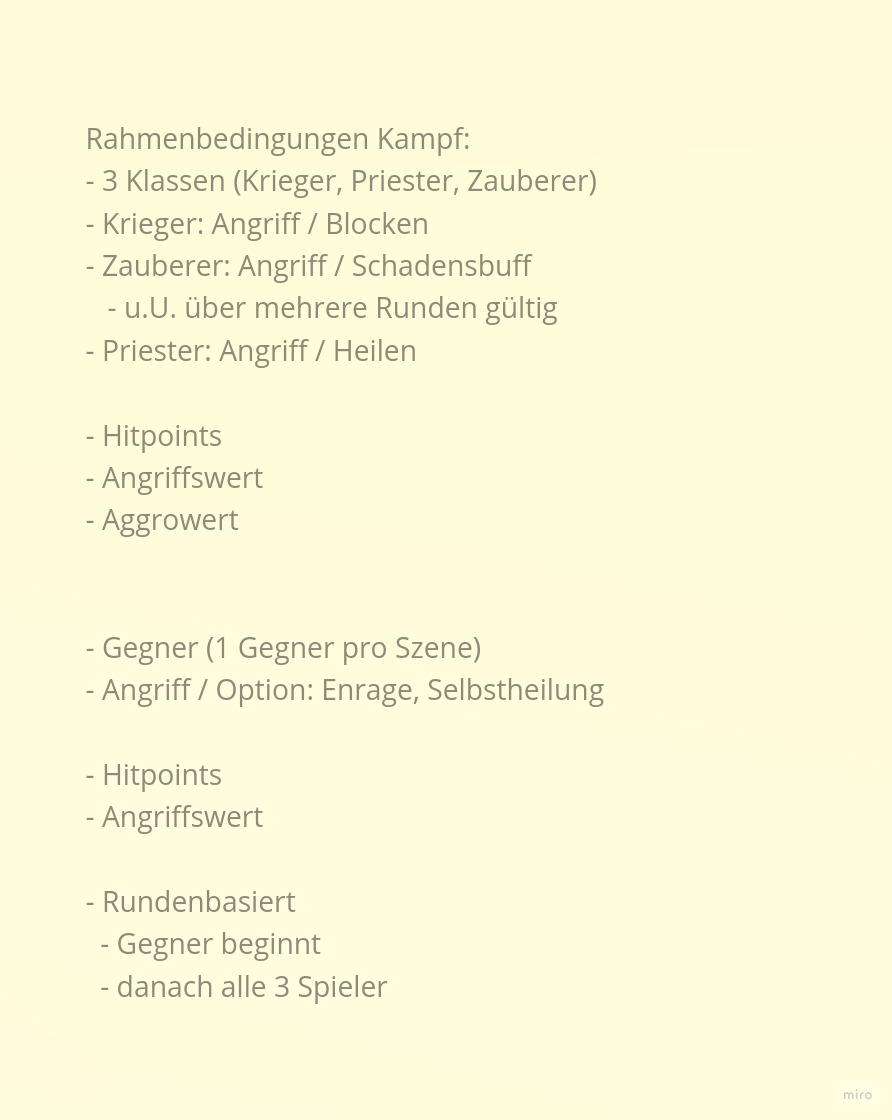
\includegraphics[width=1\textwidth]{2021-12-11-Projekt-Besprechung-Klassenbeschreibung}
\end{figure}

